\documentclass{article}
\usepackage[utf8]{inputenc}
\usepackage{graphicx}

\makeatletter
\def\@seccntformat#1{%
	\expandafter\ifx\csname c@#1\endcsname\c@section\else
	\csname the#1\endcsname\quad
	\fi}
\makeatother

\title{Distribusi Poisson}
\date{}
\author{}

\begin{document}

	\maketitle
	
	\section{Tujuan}
		1. Mempelajari karakteristik statistik peluruhan radioaktif.\\
		2. Menentukan aktivitas peluruhan preparat radioaktif.
	
	\section{Dasar Teori}
	 
		\hspace{0.35 cm} Radioaktif adalah suatu atom yang tidak stabil yang selalu melepaskan energi dan atau partikel untuk mencapai kestabilan di dalam inti atomnya. Proses pelepasan energi radiasi atau partikel ini dikenal dengan istilah peluruhan. Walaupun proses peluruhan ini bersifat acak, namun apabila jumlah partikel yang dilepaskan dalam selang waktu tertentu ternyata memiliki pola kecenderungan tertentu secara statistik.\par
		Kemungkinan suatu preparat radioaktif akan meluruh dengan melepaskan $n$ partikel dalam selang waktu $\Delta t$ tertentu dapat diperkirakan melalui pendekatan distribusi Poisson
		sebagai berikut: 
		\begin{equation}
		W_{\mu}(n) = \frac{\mu^n}{n!}\cdot e^{-\mu}
		\end{equation}
		dimana:
		\par $W_{\mu}(n)$: probabilitas peluruhan $n$ partikel
		\par $\mu$: nilai rata-rata peluruhan
		\par $n$: jumlah partikel yang meluruh \\
		
		\par Secara teoritis nilai $\mu$ sangat dipengaruhi oleh ukuran preparat dan selang waktu $\Delta t$, serta berbanding terbalik dengan waktu paruh $T_{1/2}$ dari radioaktif tersebut. 
	
		
		
		\begin{center}
			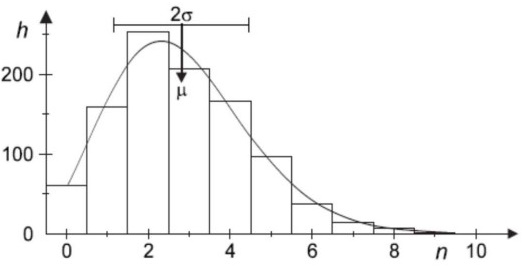
\includegraphics{./1.jpg}
			Gambar 1. Distribusi Poisson hasil pengukuran dan perhitungan. \\ Histogram: $h(n)$ dan kurva: $N.W_{\mu}$
		\end{center}
		
		\par Standard deviasi atau simpangan baku untuk distribusi Poisson dapat dihitung dengan persamaan berikut: 
		
		\begin{equation}
			\sigma = \sqrt{\mu}
		\end{equation}
		
	\section{Peralatan}
	1. 1 Unit komputer terkoneksi internet \\
	2. 1 Unit sistem kontrol \\ 
	3. 1 Set preparat radioaktif \\
	4. 1 Pencacah Geiger Muller \\
	5. 1 Sensor Cassy \\
	6. 1 GM Box \\
	
	\section{Metode Eksperimen}
	
		\hspace{0.35 cm} Pada eksperimen ini, akan dihitung frekuensi dari sejumlah $n$ partikel yang meluruh dalam selang waktu $\Delta t$ tertentu. Pengukuran tersebut dilakukan terhadap 5 jenis preparat radioaktif yang berbeda yang dihitung dengan menggunakan pencacah Geiger Muller. Setiap preparat akan dilakukan pengambilan data sebanyak $500$ data yang selanjutnya dapat ditampilkan dalam bentuk histogram. 
		
		\par Berdasarkan data tersebut, akan dihitung nilai rata-rata peluruhan $\mu$ dan simpangan bakunya $\sigma$ dengan pendekatan distribusi Poisson. Untuk preparat yang memiliki nilai rata-rata $\mu$ yang besar, dilakukan pula pendekatan distribusi normal atau Gausssian sebagai pembanding untuk membuktikan pola distribusi yang paling sesuai. 
	
	\section{Data Percobaan}
	
	\section{Pengolahan Data}
	
	\section{Pembahasan}
	
	\section{Kesimpulan}
	
	\section{Daftar Pustaka}
	
	\section{Lampiran}
	
\end{document}